\documentclass[11pt]{article}

\newcommand{\csim}{\textsf{CSIM} }
\newcommand{\nmc}{\textsf{Circuit-Tool} }
\newcommand{\lsm}{\textsf{Learning-Tool} }

%
% common packages 
%
\usepackage{graphicx}
\usepackage{color}

\PassOptionsToPackage{colorlinks=true,linkcolor=blue,citecolor=blue,urlcolor=blue}{hyperref}

\usepackage{html}

%begin{latexonly}
\usepackage{a4wide}
%\newif\ifpdf\ifx\pdfoutput\undefined\pdffalse\else\pdfoutput=1\pdftrue\fi
%\newcommand{\pdfgraphics}{\ifpdf\DeclareGraphicsExtensions{.pdf,.jpg}\else\DeclareGraphicsExtensions{.eps}\fi}
%\newcommand{\pdfgraphics}{}
%\ifpdf
%\else
% \usepackage[dvips]{hyperref}
%\fi
%end{latexonly}

\html{
  \pagecolor[gray]{1.0}
%  \newcommand{\pdfgraphics}{}
  \newcommand{\href}[2]{\htmladdnormallink{#2}{#1}}
  % we assume that the name of the hypertarget also exists as label!
  \newcommand{\hyperlink}[2]{\hyperref{#2}{}{}{#1}} 
  \newcommand{\hypertarget}[2]{#2}
}

\newcommand{\Section}[2]{\hypertarget{#2}{\section{#1}\label{#2}}}
\newcommand{\Subsection}[2]{\hypertarget{#2}{\subsection{#1}\label{#2}}}
\newcommand{\Subsubsection}[2]{\hypertarget{#2}{\subsubsection{#1}\label{#2}}}

\newcommand{\secref}[2]{\hyperlink{#1}{#2}\latex{ (Sec.~\ref{#1})}}
\newcommand{\sect}[1]{\hyperlink{#1}{Section}~\ref{#1}}
\newcommand{\figref}[1]{\hyperlink{#1}{Figure}~\ref{#1}}

\setlength{\parindent}{0em}
\setlength{\parskip}{1ex plus 0.1ex minus 0.1ex}
\setlength{\itemsep}{-0.5ex plus 0.1ex minus 0.1ex}
\setlength{\topmargin}{0cm}

%
% since we include the detailed description from doxygen we need some
% of these definitions
%
%\RequirePackage{calc}
\RequirePackage{array}
%\pagestyle{fancyplain}
%\addtolength{\headwidth}{\marginparsep}
%\addtolength{\headwidth}{\marginparwidth}
\newcommand{\clearemptydoublepage}{\newpage{\pagestyle{empty}\cleardoublepage}}
%\renewcommand{\chaptermark}[1]{\markboth{#1}{}}
\renewcommand{\sectionmark}[1]{\markright{\thesection\ #1}}
%\lhead[\fancyplain{}{\bfseries\thepage}]
%        {\fancyplain{}{\bfseries\rightmark}}
%\rhead[\fancyplain{}{\bfseries\leftmark}]
%        {\fancyplain{}{\bfseries\thepage}}
%\rfoot[\fancyplain{}{\bfseries\scriptsize Generated on Thu Nov 21 15:05:43 2002 for CSIM by Doxygen }]{}
%\lfoot[]{\fancyplain{}{\bfseries\scriptsize Generated on Thu Nov 21 15:05:43 2002 for CSIM by Doxygen }}
%\cfoot{}
\newenvironment{CompactList}
{\begin{list}{}{}}
{\end{list}}
\newenvironment{CompactItemize}
{
  \begin{itemize}
}
{\end{itemize}}
%\newcommand{\PBS}[1]{\let\temp=\\#1\let\\=\temp}
%\newlength{\tmplength}
%\newenvironment{TabularC}[1]
%{
%\setlength{\tmplength}
%     {\linewidth/(#1)-\tabcolsep*2-\arrayrulewidth*(#1+1)/(#1)}
%      \par\begin{tabular*}{\linewidth}
%             {*{#1}{|>{\PBS\raggedright\hspace{0pt}}p{\the\tmplength}}|}
%}
%{\end{tabular*}\par}
%\newcommand{\entrylabel}[1]{
%   {\parbox[b]{\labelwidth-4pt}{\makebox[0pt][l]{\textbf{#1}}\\}}}
%\newenvironment{Desc}
%{\begin{list}{}
%  {
%    \settowidth{\labelwidth}{40pt}
%    \setlength{\leftmargin}{\labelwidth}
%    \setlength{\parsep}{0pt}
%    \setlength{\itemsep}{-4pt}
%    \renewcommand{\makelabel}{\entrylabel}
%  }
%}
%{\end{list}}
%%\newenvironment{Indent}
%  {\begin{list}{}{\setlength{\leftmargin}{0.5cm}}
%      \item[]\ignorespaces}
%  {\unskip\end{list}}
%\setlength{\parindent}{0cm}
%\setlength{\parskip}{0.2cm}
%\addtocounter{secnumdepth}{1}
%\sloppy


%
% define the \objfield which is output by reggen for each registered
% field of an object.
%
\newcommand{\objfield}[6]{\item[{\normalsize \texttt{#2}} ($ #5 $) :]  {\small #6}}
\newcommand{\objfieldnu}[6]{\item[{\normalsize \texttt{#2}} :] {\small #6}}
\newcommand{\cmdref}[1]{\Subsubsection{#1}{cmd:#1}}
  
\begin{document}
%\pdfgraphics
\sloppy

%
% titlepage 
%
\latex{{
\begin{center}
  \thispagestyle{empty}
  \Huge
  
  \rule{0cm}{0cm}\\ \vfill
  
  \textbf{\csim: A Neural \textit{C}ircuit \textit{SIM}ulator}\\
  {\Large Version 1.1} \\
  \textbf{User Manual}
  
  \Large
  \vspace{3cm}
  \copyright 2002 The IGI LSM Group\\
  \url{www.lsm.tugraz.at}\\
  
  \vspace{1cm}
  
  \large
  \today
  
  \vspace{5cm}

  \vfill
  
\end{center}

% GPL
\setlength{\parindent}{0em}
\setlength{\parskip}{1ex plus 0.1ex minus 0.1ex}
\renewcommand{\baselinestretch}{0.95}
\scriptsize

This document is part of \csim Release 1.1

Copyright �2002 The IGI LSM group

\csim is free software; you can redistribute it and/or modify it
under the terms of the \href{http://www.gnu.org/copyleft/gpl.html}{GNU
  General Public License} as published by the Free Software
Foundation; either version 2, or (at your option) any later version.

\csim is distributed in the hope that it will be useful, but WITHOUT
ANY WARRANTY; without even the implied warranty of MERCHANTABILITY or
FITNESS FOR A PARTICULAR PURPOSE. See the GNU General Public License
for more details.

To get a copy of the GNU General Public License point your browser to
\url{http://www.gnu.org/copyleft/gpl.html}.

The IGI LSM group\\
Institute for Theoretical Computer Science\\
Graz University of Technology\\
Inffeldgasse 16/b, A-8010 Graz, AUSTRIA\\
\url{lsm@igi.tu-graz.ac.at}, \url{www.lsm.tugraz.at}

}
\clearpage
}
\html{\begin{flushleft}
{  \Huge  
  \textbf{\csim: User Manual}\\
  {\Large CSIM Version 1.1} \\
}

This manual is intended to describe how to use \csim from the (Matlab)
users point of view. It \emph{does not} try to explain (or give an
introduction to) the type of models which can be simulated with CSIM.
Regarding neural modeling we refer the reader to \cite{DayanAbbott:01}
and \cite{GerstnerKistler:02}.  Furthermore
\href{http://www.mathworks.com}{Matlab} programming knowledge is
assumed.

\html{This manual is also available as \href{usermanual.pdf}{printable
PDF file}.}

\latex{This manual is also available in \href{usermanual.html}{HTML
format}.}


\end{flushleft}

}

%
% table of contents
%
%%%%%%%%%%%%%%%%%%%%%%%%%%%%%%%%%%%%%%%%%%%%%%%%%%%%%%%%%%%%%%%%%%%%%%%

\setcounter{tocdepth}{3}
\tableofcontents

%%%%%%%%%%%%%%%%%%%%%%%%%%%%%%%%%%%%%%%%%%%%%%%%%%%%%%%%%%%%%%%%%%%%%%%

\Section{Preliminaries}{sec:pre}


\subsection{What is \csim?}

\csim is a tool for simulating heterogeneous networks composed of
different model neurons and synapses. This simulator is written in C++
with an MEX interface to Matlab. It is intended to simulate networks
containing up to 10.000 neurons and up to the order of a few millions
of synapses (the actual size depends of course on the amount of RAM
available on your machine).

\subsection{About this Manual}

This manual is intended to describe how to use \csim from the (Matlab)
users point of view. It \emph{does not} try to explain (or give an
introduction to) the type of models which can be simulated with CSIM.
Regarding neural modeling we refer the reader to \cite{DayanAbbott:01}
and \cite{GerstnerKistler:02}.  Furthermore
\href{http://www.mathworks.com}{Matlab} programming knowledge is
assumed.

\html{This manual is also available as \href{usermanual.pdf}{printable
PDF file}.}

\latex{This manual is also available in \href{usermanual.html}{HTML
format}.}


\subsection{Features of the current version}

\begin{description}
  
\item[Different levels of modeling] Different neuron models:
  leaky-integrate-and-fire neurons, compartmental based neurons,
  sigmoidal neurons. Different synapse models: static synapses and a
  certain model of dynamic synapses are available for spiking as well
  as for sigmoidal neurons. Spike time dependent synaptic plasticity
  is also implemented.

  
\item[Easy to use Matlab interface] Since \csim is incorporated into
  Matlab it is not necessary to learn any other script laguage to set
  up the simulation. This is all done with Matlab scripts. Furthermore
  the results of a simulation are directly returned as Matlab arrays
  and hence any plotting and analysis tools available in Matlab can
  easily be applied.
  
\item[Object oriented design] We adopted an object oriented design for
  \csim which is similar to the approaches taken in
  \href{http://www.bbb.caltech.edu/GENESIS/genesis.html}{GENESIS} and
  \href{http://www.neuron.yale.edu}{NEURON}. That is there are objects
  (e.g. a \texttt{LifNeuron} object implements the standard
  leaky-integrate-and-fire model) which are interconnected by means of
  some signal channels. The creation of objects, the connection of
  objects and the setting of parameters of the objects is controlled
  at the level of Matlab scipts whereas the actual simulation is done
  in the fast C++ core.

  
\item[Fast C++ core] Since \csim is implemented in C++ and is not as
  general as GENESIS or NEURON simulations are performed quite fast.
  We also implemented some ideas from event driven simulators like
  \href{http://www.cnl.salk.edu/~arno/spikenet/}{SpikeNet} which
  result on an average speedup of 3 (assuming an average firing rate
  of the neurons of 20\,Hz and short synaptic time constants) compared
  to a standard fixed time step simulation scheme.
  
\item[Runs on Windows and Unix (Linux)] \csim is developed on Linux but also
  runs under Windows XP (we have no more experience with Windows 98 yet, but
  it should also run there) and should in principle run on any platform for
  which Matlab is available.
  
\item[External Interface] There is an external interface which allows \csim to
  communicate with external programs. In this way one can for example control
  the miniature robot
  \href{http://www.k-team.com/robots/khepera/index.html}{Khepera} with \csim.
  This feature is not available in the Windows version.

\end{description}

\subsection{Getting and Installing \csim}

\csim is distributed under the
\href{http://www.gnu.org/copyleft/gpl.html}{GNU General Public
  License} and can be downloaded from
\url{http://www.igi.tugraz.at/csim}.


To install \csim perform the following steps:

\begin{enumerate}
\item Donwload \csim from \url{www.igi.tugraz.at/csim}
\item Unzip the file \texttt{csim-VER.zip} where \texttt{VER} stands
    for the version you have downloaded. 
    
    This will create a subdirectory \texttt{lsm} and \texttt{lsm/csim}

\item Start Matlab and change into the directory \texttt{lsm}
  
\item Run the Matlab script \texttt{install.m}.
  
\item Add the path \texttt{lsm} to the Matlab search path; e. g.
\begin{itemize}
\item  \verb#addpath('/home/jack/lsm')}# or
\item  \verb#addpath('C:\Work\Neuroscience\lsm')#.
\end{itemize}

\item Change into the directory \texttt{lsm/csim/demos} and play
  around with them.

\item Have fun using \csim !

\end{enumerate}


\subsection{Compiling \csim from the sources}
\label{sec:compile}

The instruction in this section are relevant in two cases

\begin{enumerate}

\item[a)] You do not have Linux (x86 architecture) or Windows as an operating
  system.\footnote{The compiled MEX-files (\texttt{csim.mexglx} and
\texttt{csim.dll}) which already come with \csim should run on any
Linux or Windows operationg system respectively.}

\item[b)] You are planning to add your own models written in C++ to CSIM; see
  section~\ref{sec:usermodels} for more information on this topic.

\end{enumerate}

 
%If you do not use Windows or Linux as an operating system \texttt{install.m}
%will try to compile \csim by using Matlabs \texttt{mex} utility.

Currently we support compilation using (GNU) \texttt{make} for Linux/Unix
(which most likly also works for Mac OS X) and \texttt{nmake} (Microsoft
Visual C++) for Windows (tested only with Windows XP). The corresponding
Makefiles are \verb+lsm/csim/src/Makefile+ and
\verb+lsm\csim\src\Makefile.win+.

\subsubsection*{Step by step instructions}

\begin{enumerate}

\item To compile \csim from the sources you must first setup Matlab's mex utility
properly. This can be achieved by issuing the command \verb+mex -setup+ at the
Matlab prompt. For more information on compiling MEX-files see the
\href{http://www.mathworks.com/support/tech-notes/1600/1605.html}{MEX-files
  Guide}.

\item \emph{Optional steps}: \small If you are planning to add your own models
  written in C++ to CSIM and are not using Linux or Windows you have to build
  the \texttt{reggen} tool which comes with \csim (\verb+lsm/develop/reggen+)
  for your platform.\footnote{For Linux and Windows the precompiled
    \texttt{reggen} tool is located in \texttt{lsm/develop/reggen/bin}.}

  \begin{enumerate}
      \item Go to \verb+lsm/develop/reggen+
      \item Run 
      \begin{itemize}
        \item \verb+configure; make;+ for Linux/Unix(/Mac OS)
        \item \verb+make.bat msvc+ for Windows XP with MS Visual C++ 
      \end{itemize}
    \item If this fails read \verb+lsm/develop/reggen/INSTALL+ and try to fix
      the build. In this case you will notice that \verb+reggen+ is a modified
      version of the well known tool doxygen.
  \end{enumerate}

\normalsize 

\item Edit the corresponding Makefile to meet your system configuration.

\item Goto \verb+csim/src+ and run
      \begin{itemize}
        \item \verb+make+ for Linux/Unix(/Mac OS)
        \item \verb+nmake -f Makefile.win+ for Windows (XP)
      \end{itemize}

\end{enumerate}

We do not know whether this instructions work on systems other than Windows XP
with MS Visual C++ and Linux with gcc (3.4 or higher). The
\href{http://www.mathworks.com/access/helpdesk/help/techdoc/matlab_external/matlab_external.shtml}{External
  Interfaces/API} section of the Mathworks web site and the
\href{http://www.mathworks.com/support/tech-notes/1600/1601.shtml}{Tech-Note
  1601} contain valuable information about compiler requirements for compiling
C++ MEX files.



%%%%%%%%%%%%%%%%%%%%%%%%%%%%%%%%%%%%%%%%%%%%%%%%%%%%%%%%%%%%%%%%%%%%%%%

\clearpage

\Section{A short Tutorial}{sec:start}


In this section we will introduce \csim by means of a simple example.
We will use \csim to simulate a model where a
\secref{classLifNeuron}{leaky-integrate-and-fire} neuron (LIF neuron)
is driven by a Poisson spike train which is transmitted by a
\secref{classDynamicSpikingSynapse}{dynamic synapse}.

\begin{center}
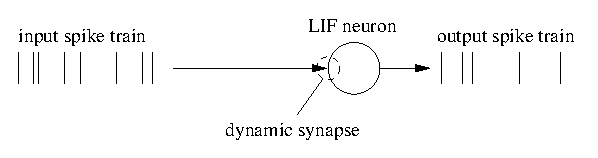
\includegraphics{first-model}
\end{center}

%\Subsection{Setting up the simulation}{subsec:setup}

\subsection{Creating Objects}

Each element/entity of the simple model we will implement, will be
simulated by a corresponding \emph{object} in \csim. The following
table shows the correspondence between the elements of the model and
the \emph{class} of the object used to simulate the element
%
\begin{center}
\begin{tabular}{l|l}
\textbf{element of model} & \textbf{class of \csim object} \\\hline
input spike train & \texttt{SpikingInputNeuron} \\
dynamic synapse & \texttt{DynamicSpikingSynapse} \\
LIF neuron & \texttt{LifNeuron}
\end{tabular}
\end{center}
%
Hence, for the simulation to run one must \secref{cmd:create}{create
  objects} of the given class:
%
\begin{tabbing}
\quad\tt>> i=csim('create','SpikingInputNeuron'); \\
\quad\tt>> s=csim('create','DynamicSpikingSynapse'); \\
\quad\tt>> n=csim('create','LifNeuron');
\end{tabbing}
%

\subsection{Object Handles}

The values \texttt{i, s}, and \texttt{n} returned by these
\secref{cmd:create}{create commands} are the \emph{indices} or
\emph{handles} to the created objects. The handles are the only means
to further access or modify existing objects.

\subsection{Setting Fields or Parameters}

Each of the created objects has several \emph{fields} which usually
correspond to a parameter of the model which is implemented by the
class of the object. To display for example all
\secref{classLifNeuron}{fields of the \texttt{LifNeuron}} object we
can use the command
%
\begin{tabbing}
\quad\tt>> csim('\hyperlink{cmd:get}{get}',n);
\end{tabbing}
%
This will yield the following output
%
\begin{verbatim}
  0 : LifNeuron
          Cm = 3e-08 (F)
          Rm = 1e+06 (Ohm)
    Vresting = -0.06 (V)
      Vreset = -0.06 (V)
       Vinit = -0.06 (V)
    Trefract = 0.003 (sec)
      Inoise = 0 (A)
     Iinject = 0 (A)
     Vthresh = -0.045 (V)
          Vm : 0 (V)
        type = 0
     nSpikes : 0
   nIncoming : 0
   nOutgoing : 0
\end{verbatim}
%
Some of the fields are parameters of the model (\texttt{Cm},
\texttt{Rm}, ...) which can be modified (denoted by the \texttt{'='})
others are internal state variables (\texttt{Vm} in this case) which
can not be changed (denoted by the \texttt{':'}) and yet other provide
auxiliary information (\texttt{nSpikes}, \texttt{nIncoming}, ...). See
the \secref{sec:clref}{Class Reference} for details about fields
of a particular object.

Suppose we want to change the absolut refractory period of the LIF
neuron \texttt{n} to be of length 2\,ms and add a noisy current of
50\,nA. This can be done with the command
%
\begin{tabbing}
\quad\tt>> csim('\hyperlink{cmd:set}{set}',n,'Trefract',0.002,'Inoise',50e-9);
\end{tabbing}
%
For the dynamic synapse \texttt{s} we choose parameters such that it
will show a depressing behaviour:
%
\begin{tabbing}
\quad\tt>> csim('\hyperlink{cmd:set}{set}',s,'W',10,'U',0.1,'D',1,'F',0.05); \\
\quad\tt>> csim('\hyperlink{cmd:set}{set}',s,'u0',0.1,'r0',1);
\end{tabbing}

\subsection{Making connections}
So far we have generated three independent objects and set
their fields to the desired values. Now we have to connect the objects
to implement our simple model. We have to connect the input \texttt{i}
to the synapse \texttt{s} and the synapse to the neuron \texttt{n}:
%
\begin{tabbing}
\quad\tt>> csim('\hyperlink{cmd:connect}{connect}',n,s); \% synapse to neuron \\
\quad\tt>> csim('\hyperlink{cmd:connect}{connect}',s,i); \% input to synapse
\end{tabbing}
%
Note the the \secref{cmd:connect}{connect command} uses the convention
that the signal destination is the first argument. Alternatively one
can use the three argument form of the command:
\begin{tabbing}
\quad\tt>> csim('\hyperlink{cmd:connect}{connect}',n,i,s); \% input to neuron via synapse
\end{tabbing}

\subsection{Recording}  The model is now fully
implemented. In addition we want to record traces of some quantities
of interest. Suppose we want record the membrane potential and the
spikes of neuron \texttt{n} as well as the postsynaptic respones (the
field \texttt{psr}) of the synapse. To do so we have to create a
\secref{classRecorder}{Recorder object} and tell this object which
fields from which objects to record. The recorder is created with the
command
%
\begin{tabbing}
\quad\tt>> r=csim('\hyperlink{cmd:create}{create}','Recorder');
\end{tabbing}
%
and the following commands tell the recorder \texttt{r} to record the
field \texttt{psr} of synapse \texttt{s} as its first trace and the
field \texttt{Vm} of neuron \texttt{n} as its second trace:
%
\begin{tabbing}
\quad\tt>> csim('\hyperlink{cmd:connect}{connect}',r,s,'psr'); \\
\quad\tt>> csim('\hyperlink{cmd:connect}{connect}',r,n,'Vm');   \\
\end{tabbing}
%
Using the special field \texttt{spikes} the same syntax will be used
to record the spikes of neuron \texttt{n} as the third trace of
recorder \texttt{r}.
\begin{tabbing}
\quad\tt>> csim('\hyperlink{cmd:connect}{connect}',r,n,'spikes');
\end{tabbing}

The following figure summarizes which objects we have created and how
they are connected:

\begin{center}
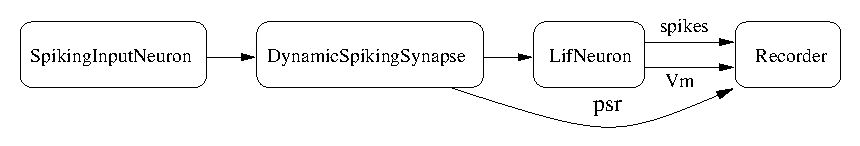
\includegraphics{first-model-csim}
\end{center}

\subsection{Setting up the input} Before we are ready to run the
simulation we have to define the spike train which should be emitted
 by the input neuron \texttt{i}. In \csim time varying
 \secref{sec:inputs}{\emph{input signals}} (analog or spiking) -- also
 called the \emph{stimulus} -- are not considered to be
 properties/attributes of some objects but are always explicitly
 specified. In the case of our example we will define a spike train
 with randomly drawn spike times (for details see \sect{sec:inputs}):
\begin{tabbing}
\quad\tt>> S.spiking = 1;                \% 1 ... spike times, 0 ... analog data\\
\quad\tt>> S.dt      = NaN;              \% resolution for analog data \\
\quad\tt>> S.idx     = i;                \% index/handle of receiving object\\
\quad\tt>> S.data    = sort(rand(1,10)); \% 10 random spikes in the interval 0 to 1 sec
\end{tabbing}

\subsection{Running the simulation} Now we are ready to run the
simulation. The command
%
\begin{tabbing}
\quad\tt>> Tsim=1; \\
\quad\tt>> csim('\hyperlink{cmd:simulate}{simulate}',Tsim,S);
\end{tabbing}
%
simulates the simple model for 1\,sec starting at time
$t=0$\footnote{In general the simulation will be continued at the time
where the last \secref{cmd:simulate}{simulate command}
stopped. However the first simulate command -- as in the case of the
example -- starts at time $t=0$. Simulation time can be reset to time
$t=0$ with the \secref{cmd:reset}{reset command}
\texttt{csim('reset');}.} with the stimulus \texttt{S}.

\subsection{Plotting the recorded traces} The traces recorded by the
recorder can be obtained by the command
\begin{tabbing}
\quad\tt>> t=csim('\hyperlink{cmd:get}{get}',r,'traces')
\end{tabbing}
which yields the output
\begin{verbatim}
t = 
    channel: [1x3 struct]
\end{verbatim}
A closer look at e.g. the first channel reveals that
\texttt{t.channel} is a struct array with a similar structure as we
have seen above for the input signal:
\begin{verbatim}
>> t.channel(1)           

ans = 

          idx: 1
    fieldName: 'psr'
         data: [1x2000 double]
      spiking: 0
           dt: 5.0000e-04
\end{verbatim}

The output indicates that \texttt{t.channel(1).data} holds the
\texttt{psr} trace (\texttt{t.channel(1).fieldName}) with a resolution
of 0.5\,ms (\texttt{t.channel(1).dt}). See the
\secref{classRecorder}{Recorder class documentation} for details abput
the structure of the trace output. Similarly \texttt{t.channel(2)}
holds the the \texttt{Vm} trace and \texttt{t.channel(3)} holds the
output spike times. Hence the following command will plot
the \texttt{psr} trace
\begin{tabbing}
\quad\tt>> plot(t.channel(1).dt:t.channel(1).dt:Tsim,t.channel(1).data);
\end{tabbing}
and the command
\begin{tabbing}
\quad\tt>> stem(t.channel(3).data,ones(size(t.channel(3).data)));
\end{tabbing}
will draw the output spike train.

Using another set of plot commands one can easily create the following
figure which shows the input, the postsynaptic response and the output
of the neuron (the voltage and the spikes)

\begin{center}
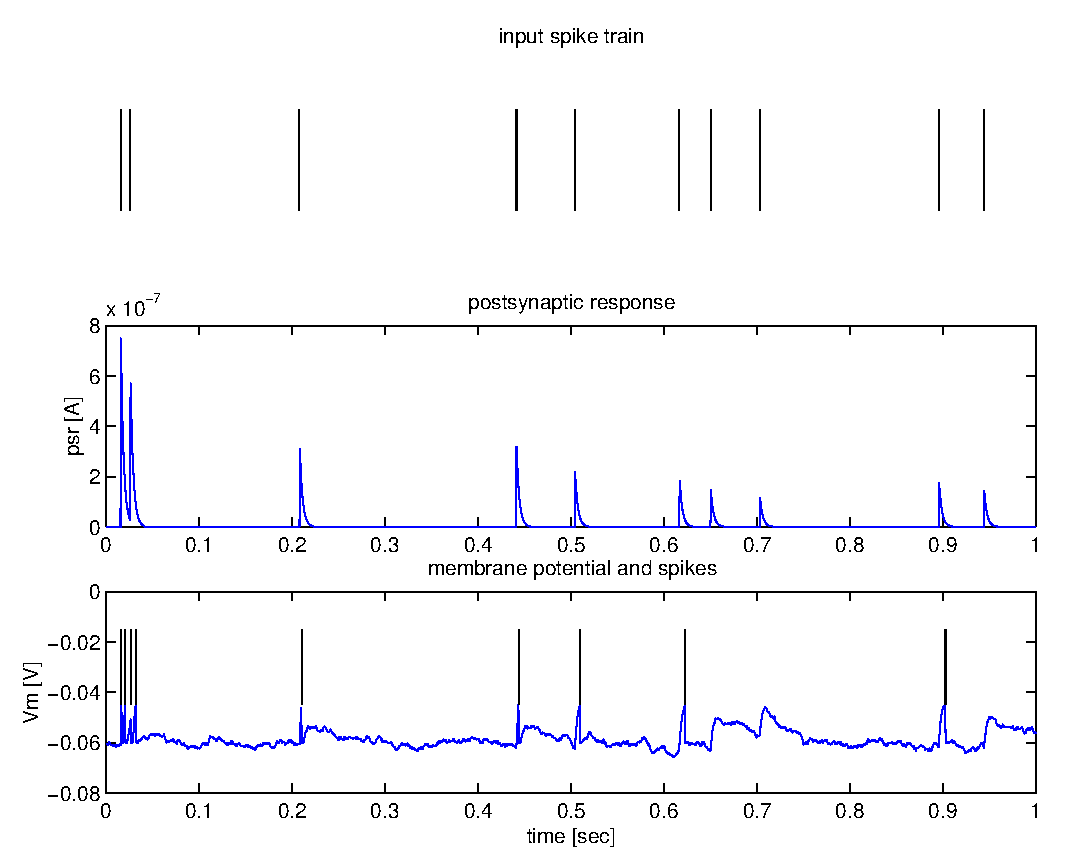
\includegraphics[width=12cm]{first-model-output}
\end{center}

The full code of this example is contained as the file
\texttt{first\_model.m} in the demo directory of the
\href{http://www.lsm.tugraz.at/csim}{\csim package}.




%%%%%%%%%%%%%%%%%%%%%%%%%%%%%%%%%%%%%%%%%%%%%%%%%%%%%%%%%%%%%%%%%%%%%%%

\Section{Input and Output}{sec:inout}

\Subsection{Input Signals}{sec:inputs}

% \Subsubsection{Single-stimulus input}{sec:singlein}

When runing a network simulation via \texttt{csim('simulate',...);}
one can specify \emph{input signals} like in the command
%
\begin{tabbing}
\quad\texttt{>> csim(\hyperlink{cmd:simulate}{'simulate'},Tsim,S);}
\end{tabbing}
%
where \texttt{S} is a struct array with the following fields:
%
\begin{itemize}
  
\item \texttt{S(i).idx} : array of handles of objects which should
  receives this signal

\item \texttt{S(i).spiking} : binary flag (0/1) which determines if
  \texttt{S(i).data} should be interpreted as spike times or as an
  analog signal
  
\item \texttt{S(i).dt} : time discretization; for analog signals
  (\texttt{S(i).spiking}=0) only
  
\item \texttt{S(i).data} : signal data: vector of the analog values
  (\texttt{S(i).spiking}=0) or spike times (\texttt{S(i).spiking}=1)

\end{itemize}
%
Note that \texttt{csim('simulate',...);} accepts an arbirary number of
such struct arrays. See \secref{cmd:simulate}{documentation of the
  simulate command}.


%\Subsubsection{Multi-stimulus input}{sec:multiin}
%
%When runing a network simulation via \texttt{csim('simulate',...);}
%one can specify a \emph{multi-stimulus} input \texttt{S} like in the command
%
%\begin{tabbing}
%\quad\texttt{>> R = csim(\hyperlink{cmd:simulate}{'simulate'},Tsim,S);}
%\end{tabbing}
%
%where \texttt{S} is a $n \times 1$ struct array of the form
%\texttt{S(i).channel} which describes the $i$-th stimulus.
%\texttt{S(i).channel} has the structure as described above.
%
%If such multi-stimulus input is specified \csim will simulate the
%current network with each of the $n$ stimuli where at the beginning of
%each stimuli the network is reset to $t=0$. The return argument
%\texttt{R} contains the recorded information of all $n$ simulations
%(see \sect{sec:multiout}).


\Subsection{Output}{sec:output}

If one simulates a network then one also wants to record the
quantities of interest. In our \secref{sec:start}{introductory
  example} we were interested in the membrane potential of the
leaky-integrate and fire neuron. \csim can record any field of any
object by means of \secref{classRecorder}{Recorder} objects. The
following code fragment shows how to set up a Recorder to record the
membrane potential (\texttt{Vm}) of a
\secref{classLifNeuron}{LifNeuron} object with handle \texttt{n}.
%
\begin{tabbing}
\quad\texttt{>> rec = csim(\hyperlink{cmd:create}{'create'},'\hyperlink{classRecorder}{Recorder}');} \\
\quad\texttt{>> csim(\hyperlink{cmd:connect}{'connect'},rec,n,'Vm');}
\end{tabbing}
%
Note that one Recorder object can record an arbitrary number of
fields from arbitrary objects.

\Subsubsection{Getting results of the last simulation}{sec:lastout}

After a network simulation via a command like
%
\begin{tabbing}
\quad\texttt{>> csim(\hyperlink{cmd:simulate}{'simulate'},Tsim,\hyperlink{sec:input}{InputSignal});}
\end{tabbing}
%
the recorded data of the \emph{the last simulation} Recorder
\texttt{rec} can be obtained by the command
\begin{tabbing}
\quad\texttt{>> R=csim(\hyperlink{cmd:get}{'get'},rec,'traces');}
\end{tabbing}
The exact structure of \texttt{R} for the recorder \texttt{rec}
depends on the value of the \secref{classRecorder}{field
\texttt{commonChannels} of the \texttt{Recorder}} object.


\paragraph{\texttt{commonChannels = 0}} In this case  (default) \texttt{R}
is a struct array with the only field \texttt{channel} which is in
turn a struct array with a similar structure as an
\secref{sec:inputs}{input signal}. That is

\begin{itemize}
  
\item \texttt{R.channel(j).idx} : handle of the object from which
  field the data was recorded
  
\item \texttt{R.channel(j).spiking} : binary flag (0/1) which
  determines if \texttt{data} should be interpreted as spike times or
  as an analog signal
  
\item \texttt{R.channel(j).dt} : time discretization; for analog
  signals   only
  
\item \texttt{R.channel(j).data} : signal data : vector of the
  analog values or spike times. Note that the data always starts at
  time $t=0$.
 
\item \texttt{R.channel(j).fieldName} : name of the recorded
    field

\end{itemize}

\paragraph{\texttt{commonChannels = 1}} In this case
\texttt{R} has two fields:
\begin{itemize}
\item \texttt{R.data} : A double array where
  \texttt{R.data(j,s)} is the $s$-th recorded value of the $j$-th
  field recorded.  Note that the data always
  starts at time $t=0$.  {\small Remark: The number of values which
    are recorded depends on the \secref{classRecorder}{field
      \texttt{dt} of the \texttt{Recorder} object}.}
  
\item \texttt{R.info} : A struct array where
  \texttt{R.info(j).idx} is the handle of the object from which
  the field \texttt{R.info(j).fieldName} is recorded.
\end{itemize}

\Subsubsection{Getting the results of a multi-stimulus simulation}{sec:multiout}

{\bf Reminder}: The command
\begin{tabbing}
\quad\texttt{>> R=csim(\hyperlink{cmd:get}{'get'},rec,'traces');}
\end{tabbing}
returns only the results of the last simulation. In the case of a
multi-stimulus simulation with stimulus array \texttt{S} of length $n$
this command returns only the result of the simulation with stimulus
\texttt{S(n)}.

To get the results of all $n$ simulations one has to use
\begin{tabbing}
\quad\texttt{>> R=csim(\hyperlink{cmd:simulate}{'simulate'},Tsim,S);}
\end{tabbing}

In that case \texttt{R} contains the results of all $n$ stimulations.
\texttt{R\{r\}(s).channel} contains the recorded data of the $r$-th
recorder during the $s$-th simulation ($1 \leq s \leq n$).
\texttt{R\{r\}(s).channel} is of the format as described in
\sect{sec:lastout}.





 
%%%%%%%%%%%%%%%%%%%%%%%%%%%%%%%%%%%%%%%%%%%%%%%%%%%%%%%%%%%%%%%%%%%%%%%
%
%\Section{Distributed Simulation}{sec:distr}
%
%\input{distributed}
% 

%%%%%%%%%%%%%%%%%%%%%%%%%%%%%%%%%%%%%%%%%%%%%%%%%%%%%%%%%%%%%%%%%%%%%%%

\Section{Additional Topics}{sec:additional}

\subsection{How the network is simulated}

\csim employs a fixed time step simulation scheme for the
integration of the differential equations involved (represented by
objects). Currently all objects use the exponential Euler method with
the same integration time step (see \sect{sec:gf}).

During each time step a certain method (\texttt{advance}) is called
for each object part of the simulation. There is a fixed schedule
which depends a) on the class of the object and b) on the time of
creation. Here is the order of the classes.
%
\begin{enumerate}
\item Neuron
\item Synapse
\item Recorder
\end{enumerate}
%
This means that all objects of classes derived from a generic Neuron
are advanced first followed by objects of classes derived from a generic
Synapse and so on.

Note that for example a more detailed neuron model (like the
\secref{classCbNeuron}{CbNeuron}) has to advance all its child objects
like ion channels.

After a \texttt{csim('simulate',...)} command returns the network is
kept in its current state at this time $t$. A further
\texttt{csim('simulate',...)}  command continues the simulation at
this time $t$. Use \texttt{csim('reset');} to reset the simulation to
time $t=0$.

Note that recorded traces you get by the appropriate
\secref{cmd:get}{get command} always start at time $t=0$.


\Subsection{Global fields}{sec:gf}

There are a few fields which determine the global (i.e. not object
specific) behavior of \csim which can be modified via the
\secref{cmd:set}{set command}:
%
\begin{tabbing}
\quad\tt>> csim('\hyperlink{cmd:set}{set}',<fieldname>,<value>); \\
\end{tabbing}
%

\subsubsection*{Read/writeable fields}


\begin{description}

\item[dt] The integration time step used by all objects

\item[randSeed] The seed value for the random number generator

\item[verboseLevel] How much stuff should be written to the
  console window (no effect yet!).
  
\item[nThreads] Number of threads to use for simulation (no
  effect yet!). The multi-threaded version of \csim is currently under
  development.

\item[spikeOutput] Flag: 1 ... always output spikes as last cell element, 0 do not
  output spikes (obsolete).

\end{description}

\subsubsection*{The following fields are read-only:}

\begin{description}

\item[t] The current virtual (simulation) time
  
\item[step] The current time step; i.e.  \texttt{step=t/dt};

\end{description}

\subsection{Event driven simulation}

Since in a typical simulation the firing rate of the neurons is about
30\,Hz and the time constant of a synaptic current is typically about
3\,ms most of the time a synapse is ``idle''. This observation
encouraged us to implement some ideas of event driven simulators like
\href{http://www.cnl.salk.edu/~arno/spikenet/}{SpikeNet}\latex{\footnote{\url{http://www.cnl.salk.edu/~arno/spikenet/}}}:
We decided to cut off the very far tail of the exponential decaying
synaptic responses (after 5 time constants) and remove those synapses
from the list of active synapses (which are advanced every time step).
A synapse is re-activated if it receives a further spike. For large
networks with lots of synapses these idea results in an average
speed-up of 2 to 3.


 
%%%%%%%%%%%%%%%%%%%%%%%%%%%%%%%%%%%%%%%%%%%%%%%%%%%%%%%%%%%%%%%%%%%%%%%

\Section{Adding your own C++ model classes to \csim}{sec:usermodels}

This section describes how a user can add its own models to CSIM at the C++
level.

\subsection{Recipe}

\begin{enumerate}
  
\item Create a copy of that existing model which is closest to that you wish
  to implement in the directory \verb+lsm/csim/src+. In the following we
  assume that the related files are called \verb+MyModel.h+ and
  \verb+MyModel.cpp+.

\item Implement your model.

\item Add you model to CSIM:
\begin{itemize}
\item Linux/Unix/: Add \verb+MyModel.o+ to the list of objects in the \verb+Makefile+.
\item Windows: Add  \verb+MyModel.obj+ to the list of objects in the \verb+Makefile.win+.
\end{itemize}

\item Compile CSIM:

\begin{itemize}
\item Linux/Unix/: Run the command \verb+make+
\item Windows: Run the command \verb+nmake -f Makefile.win+
\end{itemize}

\item Use your model!

\end{enumerate}

\subsection{Details}

During the compilation of CSIM a tool called \verb+reggen+ is used to generate
wrapper code which allows you to access the parameters of your model from the
Matlab level. This frees you from the tedious work of writing lots of code
for getting and setting such fields. For more details about this issue see the
subsection~\ref{sec:fields}.

If you are not using Linux or Windows you have to build the \texttt{reggen}
tool which comes with \csim (\verb+lsm/develop/reggen+) for your
platform.\footnote{For Linux and Windows the precompiled \texttt{reggen} tool
  is located in \texttt{lsm/develop/reggen/bin}.}

\begin{enumerate}
\item Go to \verb+lsm/develop/reggen+
\item Run 
  \begin{itemize}
  \item \verb+configure; make;+ for Linux/Unix(/Mac OS)
  \item \verb+make.bat msvc+ for Windows XP with MS Visual C++ 
  \end{itemize}
\item If this fails read \verb+lsm/develop/reggen/INSTALL+ and try to fix
  the build. In this case you will notice that \verb+reggen+ is a modified
  version of the well known tool doxygen.
\end{enumerate}

\subsection{Hints for adding user defined models}

\begin{itemize}

\item Don't forget the line \verb+DO_REGISTERING+ in the class declaration of
  you model.

\item Use doxygen comments to document your model.

\end{itemize}

\Subsection{Setting and getting field values of objects}{sec:fields}

\hypertarget{fields}{}\section{Setting and getting field values of objects}\label{fields}
At the Matlab level CSIM allows you to set and get values of fields of objects by means of the commands



\footnotesize\begin{verbatim}  v=csim('get',o,fieldname)
  csim('set',o,fieldname,value)
\end{verbatim}
\normalsize


where {\tt o} is the handle of the object returned by



\footnotesize\begin{verbatim}  o=csim('create',classname)
\end{verbatim}
\normalsize


and {\tt fieldname} is a string identifying the field (i.e. the name of the field).\hypertarget{fields_fields_implementation}{}\subsection{Implementaion}\label{fields_fields_implementation}
We implemented this mechanism using four classes:

\begin{itemize}
\item \hyperlink{classcsimClass}{csim\-Class} : the base classes of all classes in CSIM which implements the basic set and get methodes for accessable fields\end{itemize}


\begin{itemize}
\item \hyperlink{classcsimClassInfoDB}{csim\-Class\-Info\-DB} : a container (of \hyperlink{classcsimClassInfo}{csim\-Class\-Info} objects) where information about all the (at the matlab level) available classes is stored\end{itemize}


\begin{itemize}
\item \hyperlink{classcsimClassInfo}{csim\-Class\-Info} : which stores information (accessible fields, description) about a certain class\end{itemize}


\begin{itemize}
\item \hyperlink{classcsimFieldInfo}{csim\-Field\-Info} : stores information about a certain field of a given class\end{itemize}
\hypertarget{fields_fields_reg}{}\subsubsection{Registering classes and fields}\label{fields_fields_reg}
To make the set and get methodes of a class derived from \hyperlink{classcsimClass}{csim\-Class} work one has to register this class via \hyperlink{classcsimClassInfoDB_a2}{csim\-Class\-Info\-DB::register\-Csim\-Class()} and then to register each member variable which we want to be an accessable field via \hyperlink{classcsimClassInfo_z1_0}{csim\-Class\-Info::register\-Field()} .

Class member variable of the types

\begin{itemize}
\item {\tt double} and {\tt double} $\ast$\item {\tt float} and {\tt float} $\ast$\item {\tt int} and {\tt int} $\ast$\end{itemize}


can be made accessible fields.

Each field has the following associated information (see \hyperlink{classcsimFieldInfo}{csim\-Field\-Info} )\begin{itemize}
\item access : \hyperlink{csimclass_8h_a7}{READWRITE} or \hyperlink{csimclass_8h_a6}{READONLY}\item units\item lower and upper bound\item size : the number of elements if the field is of type {\tt float} $\ast$, {\tt double} $\ast$, or {\tt int} $\ast$\end{itemize}
\hypertarget{fields_reggen}{}\subsubsection{reggen}\label{fields_reggen}
It woul be a tedious work to code all the \hyperlink{classcsimClassInfoDB_a2}{csim\-Class\-Info\-DB::register\-Csim\-Class()} and \hyperlink{classcsimClassInfo_z1_0}{csim\-Class\-Info::register\-Field()} function calls by hand. So we decided to generate it automatically from the source code. We use a tool named {\tt reggen} (a quick and dirty hack based on doxygen) to gather the infomation from the source code and its doxygen style documentation. {\tt reggen} writes all relevant function calls to register fields an classes to {\tt registerclass.i} \hypertarget{fields_def}{}\paragraph{Default behaviour of $\backslash$c reggen}\label{fields_def}
\begin{itemize}
\item {\tt public} class member variables are registered as \hyperlink{csimclass_8h_a7}{READWRITE} fields\end{itemize}


\begin{itemize}
\item {\tt protected} class member variables are registered as \hyperlink{csimclass_8h_a6}{READONLY}\end{itemize}


\begin{itemize}
\item {\tt private} class member variables are not registered.\end{itemize}


\begin{itemize}
\item no units are assumed (i.e. a dimensionless field)\end{itemize}


\begin{itemize}
\item lower and upper bound are set to -Inf and +Inf respectively\end{itemize}


\begin{itemize}
\item an warning is issued if no size information is given for arrays\end{itemize}


\begin{itemize}
\item the brief {\tt doxygen} comment is used as descriptio of the field\end{itemize}


\begin{itemize}
\item the brief {\tt doxygen} comment of a class is used as its description\end{itemize}
\hypertarget{fields_spec}{}\paragraph{Specifying information for use by reggen}\label{fields_spec}
If you want to register a class you just put the macro {\tt \hyperlink{csimclass_8h_a8}{DO\_\-REGISTERING}} somewhere in the class definition.

For each of the member variables where you want to change the default behaviour of {\tt reggen} you have to put a {\tt doxygen} brief comment where you specify the relevant information.\hypertarget{fields_e1}{}\subparagraph{Example 1}\label{fields_e1}
Make the float variable {\tt S} a read-writable field with units Volt and a lower and upper bound of -1 and +1 respectively: 

\footnotesize\begin{verbatim}  //! A voltage scale factor [readwrite; units=Volt; range=(-1,1);]
  float S;
\end{verbatim}
\normalsize
\hypertarget{fields_e2}{}\subparagraph{Example 2}\label{fields_e2}
Make the double variable {\tt $\ast$A} a read-only field with 20 elements, units Ohm, and a lower and upper bound of -100 and +100 respectively: 

\footnotesize\begin{verbatim}  //! A voltage scale factor [readonly; size=20; units=Ohm; range=(-100,100);]
  double *A;
\end{verbatim}
\normalsize
\hypertarget{fields_src}{}\paragraph{Source code of reggen}\label{fields_src}
\begin{itemize}
\item Currently reggen is maintained in {\tt lsm/develop/reggen} .\item The relevant source file is {\tt lsm/develop/reggen/src/defgen}.cpp .\item The binaries are {\tt lsm/develop/reggen/bin/reggen} for Linux and {\tt lsm/develop/reggen/bin/reggen}.exe for windows.\item To compile reggen under Linux type\end{itemize}




\footnotesize\begin{verbatim}  cd lsm/develop/reggen; ./configure; make
\end{verbatim}
\normalsize


\begin{itemize}
\item To compile reggen under Windows XP with MS Visual C++ type\end{itemize}




\footnotesize\begin{verbatim}  cd lsm/develop/reggen; make.bat msvc
\end{verbatim}
\normalsize
 


 
%%%%%%%%%%%%%%%%%%%%%%%%%%%%%%%%%%%%%%%%%%%%%%%%%%%%%%%%%%%%%%%%%%%%%%%

\clearpage

\Section{\csim command reference}{sec:cmdref}


The common form of all \csim commands is 
\begin{verbatim}
  csim(command,...);
\end{verbatim}
where \texttt{command} is one of the following strings:

\begin{itemize}
\setlength{\itemsep}{-0.8ex plus 0.1ex minus 0.1ex}
\setlength{\parsep}{0.0ex plus 0.1ex minus 0.1ex}
\item \texttt{\secref{cmd:create}{'create'}} : Create an object of a certain class
\item \texttt{\secref{cmd:set}{'set'}} : Set fields of an object
\item \texttt{\secref{cmd:connect}{'connect'}} : Connect objects
\item \texttt{\secref{cmd:get}{'get'}} : Get field values of an object
% \item \texttt{\secref{cmd:access}{'access'}} : Set default network
\item \texttt{\secref{cmd:reset}{'reset'}} : Reset the simulation to $t=0.0$
\item \texttt{\secref{cmd:simulate}{'simulate'}} : Simulate the network
\item \texttt{\secref{cmd:export}{'export'}} : Export the network for saving it
\item \texttt{\secref{cmd:import}{'import'}} : Import a loaded network
\item \texttt{\secref{cmd:destroy}{'destroy'}} : Destroy/delete the current netork
\item \texttt{\secref{cmd:list}{'list'}} or \texttt{\secref{cmd:list}{'ls'}} List various items
\item \texttt{\secref{cmd:version}{'version'}} : Print out a version string
% \item \texttt{\secref{cmd:pvm}{'pvm'}} : Initialize distributed simulation
\end{itemize}

A detailed description of each of the commands follows. 

%\subsection{Multiple Networks}
%
%\csim is capable of holding more then one network at a time. There are
%two ways of specifing on which network a command should operate.
%
%\begin{itemize}
%\item For each command of the form \texttt{csim(command,...);} the
%form \texttt{csim(netIdx,command,...);} exists which allows you to
%explicitly specify the network to operate on.
%
%\item If \texttt{csim(command,...);} is used the \emph{default
%    network} is used. The default network is set using the command
%  \texttt{csim('access',netIdx);}.
%\end{itemize}
%
%\cmdref{access}
%
%\begin{itemize}
%  
%\item \texttt{idx=csim('access',netIdx);} makes the network specified
%  by \texttt{netIdx} the default network and returns that value.%
%
%\item \texttt{csim('access',netIdx);} makes the network specified
%  by \texttt{netIdx} the default network and prints that value.
%
%\item \texttt{idx=csim('access');} returns the index of the default
%  network.
%
%\item \texttt{csim('access');} prints the index of the default%
%
%\end{itemize}


\subsection{Setting up a network simulation}

\cmdref{create}

\begin{itemize}
  
%\item \texttt{idx=csim('create','Network');} creates a new network and
%  returns the \emph{index} or \emph{handle} for the created network.
%  The new network is the new default network; see command
%  \secref{cmd:access}{access}.

\item \texttt{idx=csim('create',class);} creates an object of the class
  specified by the string \texttt{class} and returns a \texttt{uint32}
  \emph{index} or \emph{handle} for the created object. This
  index/handle is the only means to access the created object.
  
\item \texttt{idx=csim('create',class,N);} creates \texttt{N} objects
  of the class specified by the string \texttt{class} and returns a
  \texttt{uint32} vector of indices/handles for the created objects.

\end{itemize}

The handles returned by \texttt{idx=csim('create',...);} are used to
identify the objects later in \texttt{'set'}, \texttt{'get'} and
\texttt{'connect'} calls.

See the \secref{sec:clref}{Class Reference} for a full description of
all available classes.

\cmdref{set}

\begin{itemize}
  
\item \texttt{csim('set',field,value);} sets the
  \secref{sec:gf}{network field} specified by the string
  \texttt{field} to \texttt{value}.
  
\item \texttt{csim('set',idx,field,value);} sets the field specified
  by the string \texttt{field} of the object with index/handle
  \texttt{idx} to \texttt{value}. \texttt{idx} can also be a vector
  of indices/handles of objects of the same class.
  
If \texttt{idx} is a vector and \texttt{value} is a scalar then the
fields of all objects are set to \texttt{value}.

If \texttt{idx} and \texttt{value} are vectors of the same size then
the field \texttt{field} of all objects \texttt{idx(i)} is set to
\texttt{value(i)}.

\item \texttt{csim('set',idx,f1,v1,f2,f2,...,fn,vn);} sets the fields
  specified by the strings \texttt{f1}, \texttt{f2}, ..., \texttt{fn}
  of the object with index/handle \texttt{idx} to the values
  \texttt{v1}, \texttt{v2}, ... \texttt{vn}. \texttt{idx} and
  \texttt{v1}, \texttt{v2}, ... \texttt{vn} can also be vectors.

\end{itemize}


\cmdref{connect}

\begin{itemize}
  
\item\texttt{csim('connect',dstIdx,srcIdx);} sets up a signal flow
  from the source \texttt{srcIdx} object (e.g. a synapse) to the
  destination object \texttt{dstIdx} (e.g. the postsynaptic neuron)
  where \texttt{dstIdx} and \texttt{srcIdx} are indices/handles to
  objects.
  
  \texttt{dstIdx} and \texttt{srcIdx} can also be vectors. In that
  case for each \texttt{i=1:length(srcIdx);} a signal flow
  $\mathtt{dstIdx(i)} \leftarrow \mathtt{srcIdx(i)}$ is set up.
  
\item\texttt{csim('connect', dstIdx, srIdx, viaIdx);} for each
  \texttt{i=1:length(srcIdx);} a signal flow of the form
  $\mathtt{dstIdx(i)} \leftarrow \mathtt{viaIdx(i)} \leftarrow
  \mathtt{srcIdx(i)}$ is set up where \texttt{dstIdx},
  \texttt{srcIdx}, and \texttt{viaIdx} are vectors of the same length
  of indices/handles to objects.
  
\item\texttt{csim('connect',recIdx,objIdx,fieldName);} connects the
  object with handle \texttt{objIdx} to the recorder with handle
  \texttt{recIdx}. The recorder \texttt{recIdx} will then record a
  trace of the values of the field \texttt{fieldName} of the objects
  specified by the vector of hadles \texttt{objIdx}.

\end{itemize}

\subsection{Running the network simulation}

\cmdref{reset}

\texttt{csim('reset');} resets the simulation time $t$ back to
$t=0.0$.

\Subsubsection{simulate}{cmd:singlesim}
\label{cmd:simulate}

\begin{itemize}
  
\item \texttt{csim('simulate',Tsim,InputSignals);} runs the network
  simulation for \texttt{Tsim} seconds starting at the time where the
  last simulate command stopped with \secref{sec:inputs}{input signals
    \texttt{InputSignals}}.
  
\item \texttt{csim('simulate',Tsim,I1,I2,...,In);} same as above but
  with input signals \texttt{I1} to \texttt{In}. There is no special
  meaning in the ordering of the input signals. It is equvivalent to
  concatenate \texttt{I1} to \texttt{In} into one struct array and
  pass this array as the single input signal.
  
\item \texttt{R=csim('simulate',Tsim,InputSignals);}\\ same as
  \texttt{csim('simulate',Tsim,InputSignals);} but in addition returns
  the cell array \texttt{R} which holds the \secref{sec:output}{output
    (traces) of all Recorder objects}.
  
\item \texttt{R=csim('simulate',Tsim,I1,I2,...,In);}\\ same as
  \texttt{csim('simulate',Tsim,I1,I2,...,In);} but in addition returns
  the cell array \texttt{R} which holds the \secref{sec:output}{output
    (traces) of all Recorder objects}.

\item \texttt{R=csim('simulate',Tsim,I1,I2,...,In);}\\ same as
  \texttt{csim('simulate',Tsim,I1,I2,...,In);} but in addition returns
  the cell array \texttt{R} which holds the \secref{sec:output}{output
    (traces) of all Recorder objects}.


\end{itemize}

%\Subsubsection{Multi-stimulus simulate}{cmd:singlemulti}
%
%\texttt{R=csim('simulate',Tsim,S);} runs $n$ network simulations for
%\texttt{Tsim} sec. The network is reset to $t=0$ before each
%simulation.
%
%The $n$ simulations are determined by the $n \times 1$ strucht array
%\texttt{S} where \texttt{S(i).channel} specifies the stimulus for the
%$i$-th simulation (see \sect{sec:multiin}).
%
%\texttt{R} contains the reorded values of all $n$ simulations (see
%\sect{sec:multiout}).
%  
%If the \secref{sec:distr}{distributed simulation} is on (see command
%\secref{cmd:pvm}{pvm}), the $n$ simulations will be carried out in
%parallel.
%
%\subsection{Initializing PVM}
%
%\cmdref{pvm}

\subsection{Saving, loading and deleting networks }

\cmdref{export}

The command
\begin{verbatim}
  net = csim('export');
\end{verbatim}
produces a struct array \texttt{net} which contains all information
about the current network simulation which is needed to set up the
simulation. Using \texttt{save file.mat net} you can save the whole
network simulation.

NOTE: The struct array \texttt{net} returned by
\texttt{net=csim('export');} is only intended to be saved to disk for
later use by \texttt{csim('import',net);} and does not have a human
readable form.

\cmdref{import}

The command
\begin{verbatim}
  csim('import',net);
\end{verbatim}
allows you to set up a network simulation from the struct array
\texttt{net} which has previously been generated by \texttt{net =
  csim('export');}. In combination with the matlab command
\texttt{load} this \csim command serves the purpose of loading a
simulation from disk.

If the current network (either explicitly specified or default
network) does not contain any objects the \texttt{net} will be
imported into that network. If there are already objects a new network
will be created and and \texttt{net} will be imported to that.

NOTE: The struct array \texttt{net} returned by
\texttt{net=csim('export');} \emph{does not} contain information about
the current state of the simulation at time $t$.  \emph{Hence it is
  only possible to start simulation based on such an arry at time
  $t=0.0$.}

\cmdref{destroy}

\texttt{csim('destroy');} all the networks.

\subsection{Displaying/Getting information}

\cmdref{get}

\begin{itemize}

  \item \texttt{csim('get');} diplays the values of the \secref{sec:gf}{global fields}

  \item \texttt{v=csim('get',field);} return the value of the
    \secref{sec:gf}{global field} specified by the string \texttt{field}

  \item \texttt{csim('get',idx);} displays the values of all fields of the
    object specified by the array index/handle \texttt{idx}

  \item \texttt{v=csim('get',idx,field);} returns a double array
   \texttt{v} where \texttt{v(:,i)} contains the values of the field
   \texttt{field} of the object with index/handle \texttt{idx(i)}.

 \item \texttt{o=csim('get',idx,'struct');} return a struct array
   describing the object specified by the index/handle
   \texttt{idx(1)}:

   \begin{itemize}
   \item \texttt{o.className} : String containing the name of class of object
   \item \texttt{o.spiking} : Double value which is 1 if the object is a
     spike emitting object (0 otherwise)
   \item \texttt{o.fields} : Cell array of strings containing the field
     names of the object
   \item and all fields with its values.
   \end{itemize}
   
 \item \texttt{[incomming,outgoing]=csim('get',idx,'connections');}
   returns the indices/handles of the incomming (i.e. input
   delivering) and outgoing (i.e. output receiving) objects of the
   object specified by the index/handle \texttt{idx}. This is
   currently only implemented for Synapses and Neurons.
   
 \item \texttt{R=csim('get',recorder\_idx,'traces');} returns the
   traces of the fields recorded by the
   \secref{classRecorder}{Recorder} object with handle
   \texttt{recorder\_idx} during the \emph{last simulation}. See the
   \secref{classRecorder}{Recorder documentation} for details about
   the format of \texttt{R}.

\end{itemize}

\cmdref{list}

\begin{itemize}
  
\item \texttt{csim('list');} and \texttt{csim('list','classes');}
  print a list of all available classes
  
\item \texttt{csim('list','classes','-fields');} prints a list of all
  available classes with information about the fields of each class.
  Read/writeable fields are marked by a '\texttt{=}' between the field
  name and its description, wheres a '\texttt{:}' denotes a read-only
  field.

\item \texttt{csim('list','objects');}  prints a list of all created
  objects

\item \texttt{csim('list','objects','-fields');} prints a list of all
  created objects and the values of its fields. Read/writeable fields
  are marked by a '\texttt{=}' between the field name and its value,
  wheres a '\texttt{:}' denotes a read-only field.

\item \texttt{csim('list','networks');}  prints a list of all networks

\item \texttt{csim('list','networks','-fields');} prints a list of all
  networks and the values of its fields. Read/writeable fields
  are marked by a '\texttt{=}' between the field name and its value,
  wheres a '\texttt{:}' denotes a read-only field.

\end{itemize}

Not that instead of \texttt{'list'} one can use \texttt{'ls'} as a
shortcut.

\cmdref{version}

\begin{itemize}
\item \texttt{csim('version')} prints a version string
\item \texttt{v=csim('version');} returns the version string
\end{itemize}

%%% Local Variables: 
%%% mode: latex
%%% TeX-master: t
%%% End: 


%%%%%%%%%%%%%%%%%%%%%%%%%%%%%%%%%%%%%%%%%%%%%%%%%%%%%%%%%%%%%%%%%%%%%%%


\Section{\csim model classe reference}{sec:clref}

\input{um_class_ref}

%%%%%%%%%%%%%%%%%%%%%%%%%%%%%%%%%%%%%%%%%%%%%%%%%%%%%%%%%%%%%%%%%%%%%%%

\bibliographystyle{apalike}

\bibliography{references}

\end{document}
